\subsection{On the mehcanism of modes $A'$ and $QS$}

\begin{figure}
  \centering
  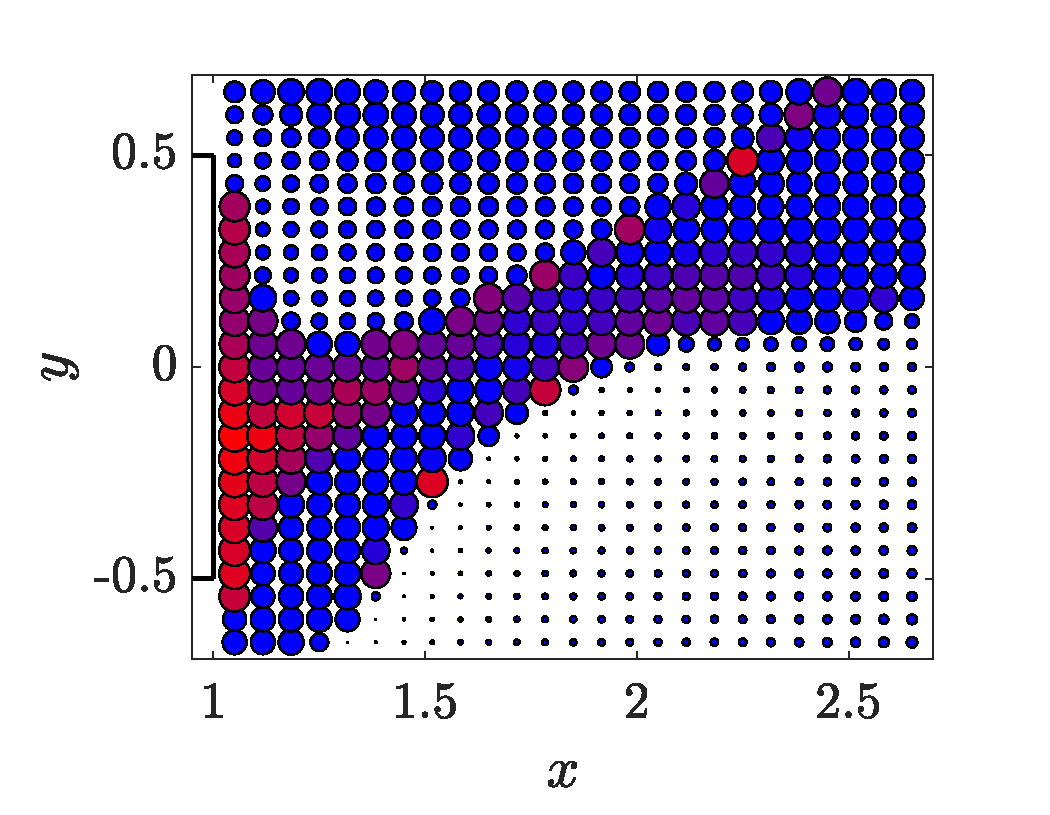
\includegraphics[width=0.49\textwidth]{./fig/LagTrac/part_AR1_Re200.eps}
  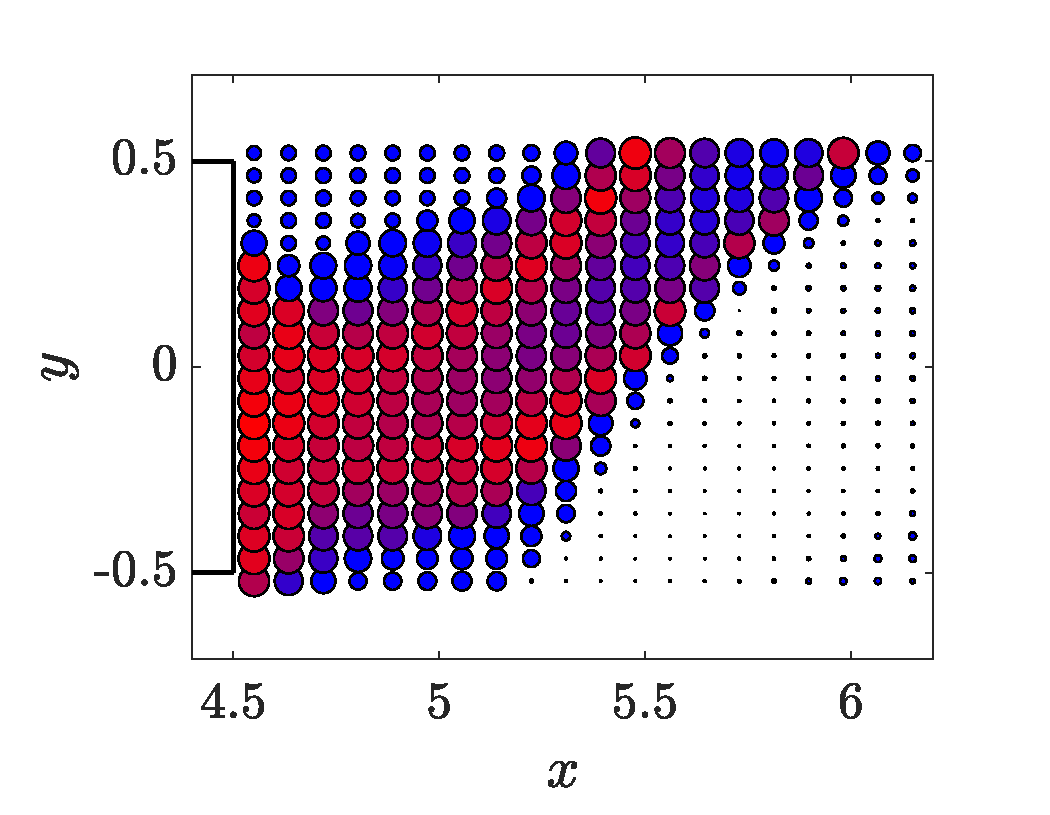
\includegraphics[width=0.49\textwidth]{./fig/LagTrac/part_AR4p5_Re410.eps}
  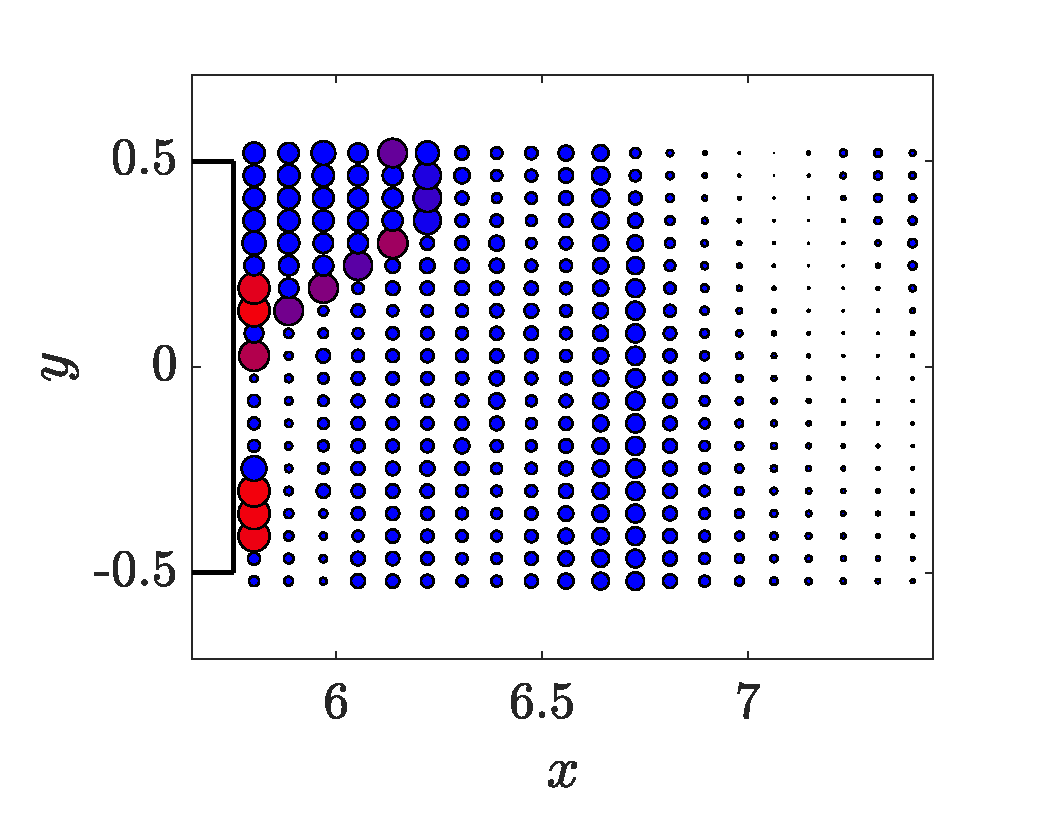
\includegraphics[width=0.49\textwidth]{./fig/LagTrac/part_AR5p75_Re550.eps}
  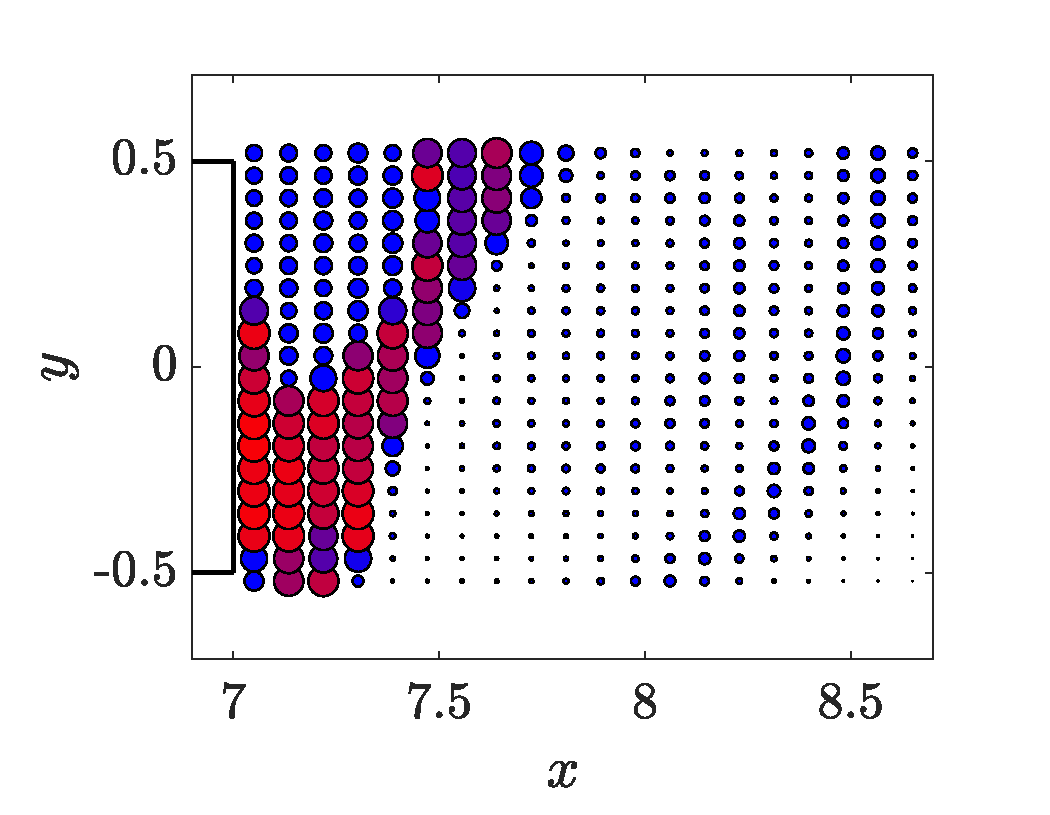
\includegraphics[width=0.49\textwidth]{./fig/LagTrac/part_AR7_Re500.eps}  
  \caption{XX AUMENTARE IL RANGE INVESTIGATO XX. PER AR=1 DOBBIAMO INVESTIGARE QUELLO CHE ABBIAMO ANCHE SOPRA AL RETTANGOLO XX}
  \label{fig:part_res}
\end{figure}    

\begin{figure}
  \centering
  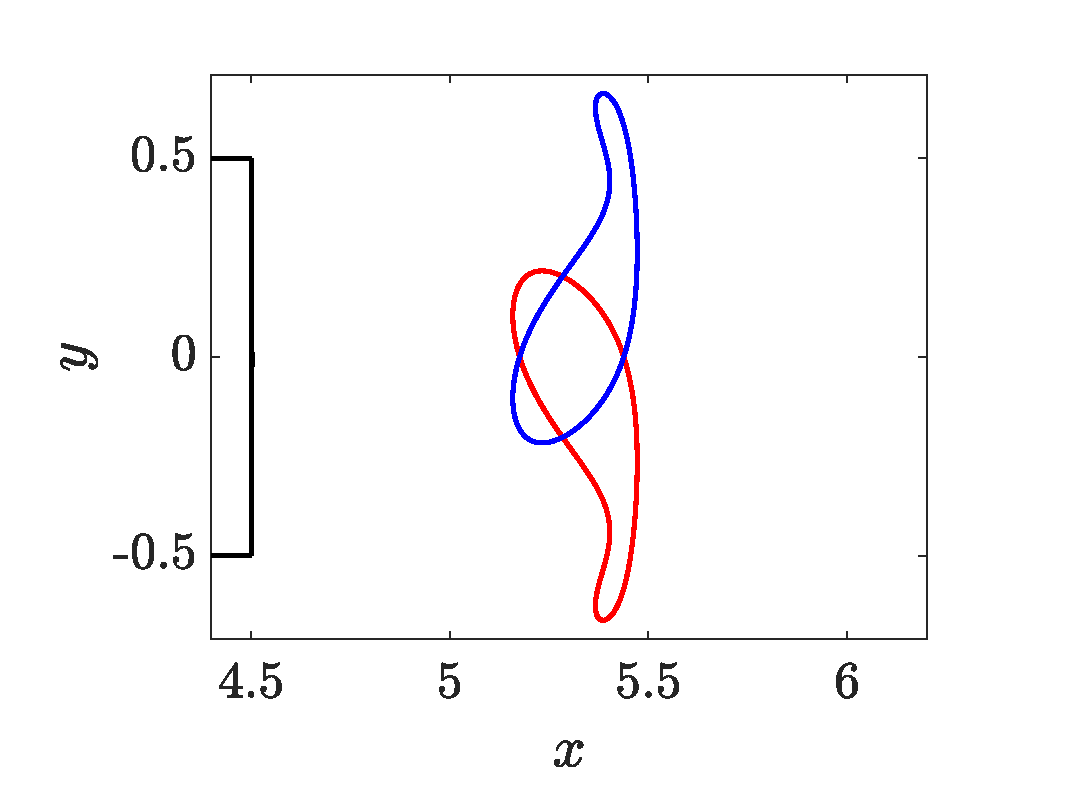
\includegraphics[width=0.49\textwidth]{./fig/LagTrac/orb_AR4p5_Re410.eps}   
  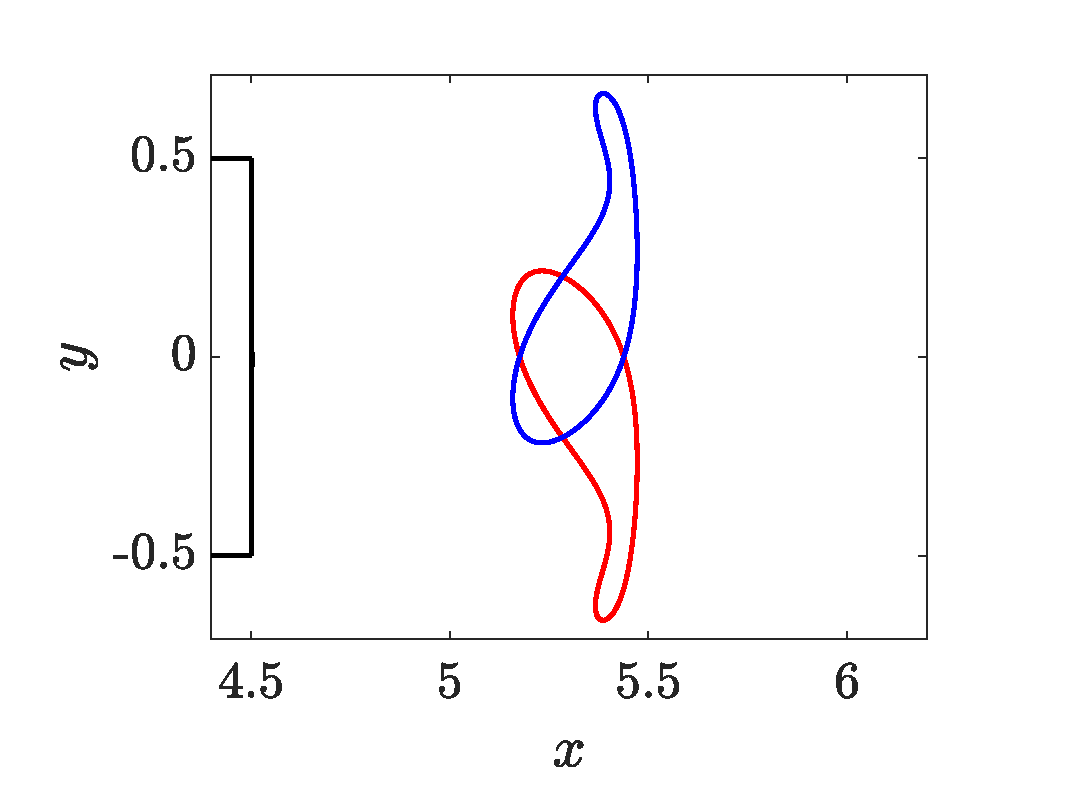
\includegraphics[width=0.49\textwidth]{./fig/LagTrac/orb_AR4p5_Re410.eps} 
  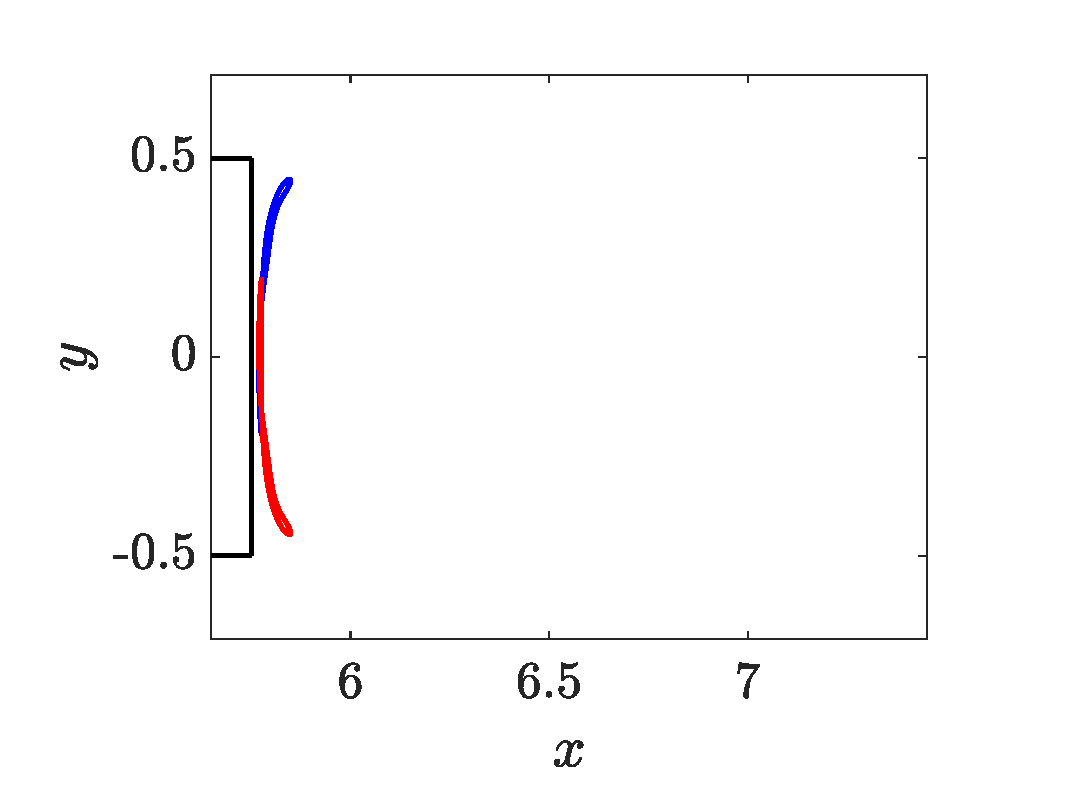
\includegraphics[width=0.49\textwidth]{./fig/LagTrac/orb_AR5p75_Re550.eps}
  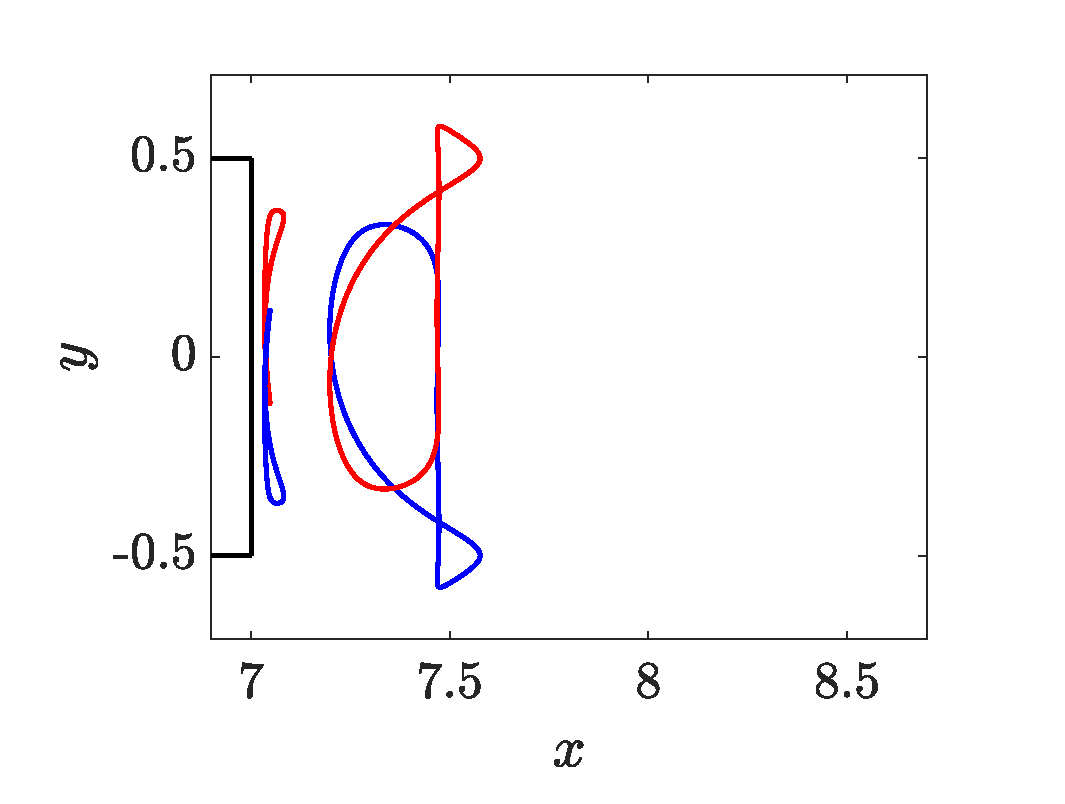
\includegraphics[width=0.49\textwidth]{./fig/LagTrac/orb_AR7_Re500.eps}
  \caption{XX AUMENTARE IL RANGE INVESTIGATO XX}
  \label{fig:part_res}
\end{figure}

XX POSSIAMO FARE ENDOGENEITY PER STUDIARE LA SCIA STORTA CHE VEDIAMO PER $\AR=4.5$ QUANDO SI STABILIZZA? POSSIAMO VEDERE CHI NE DETERMINA LA FREQUENZA XX

\begin{figure}
  \centering
  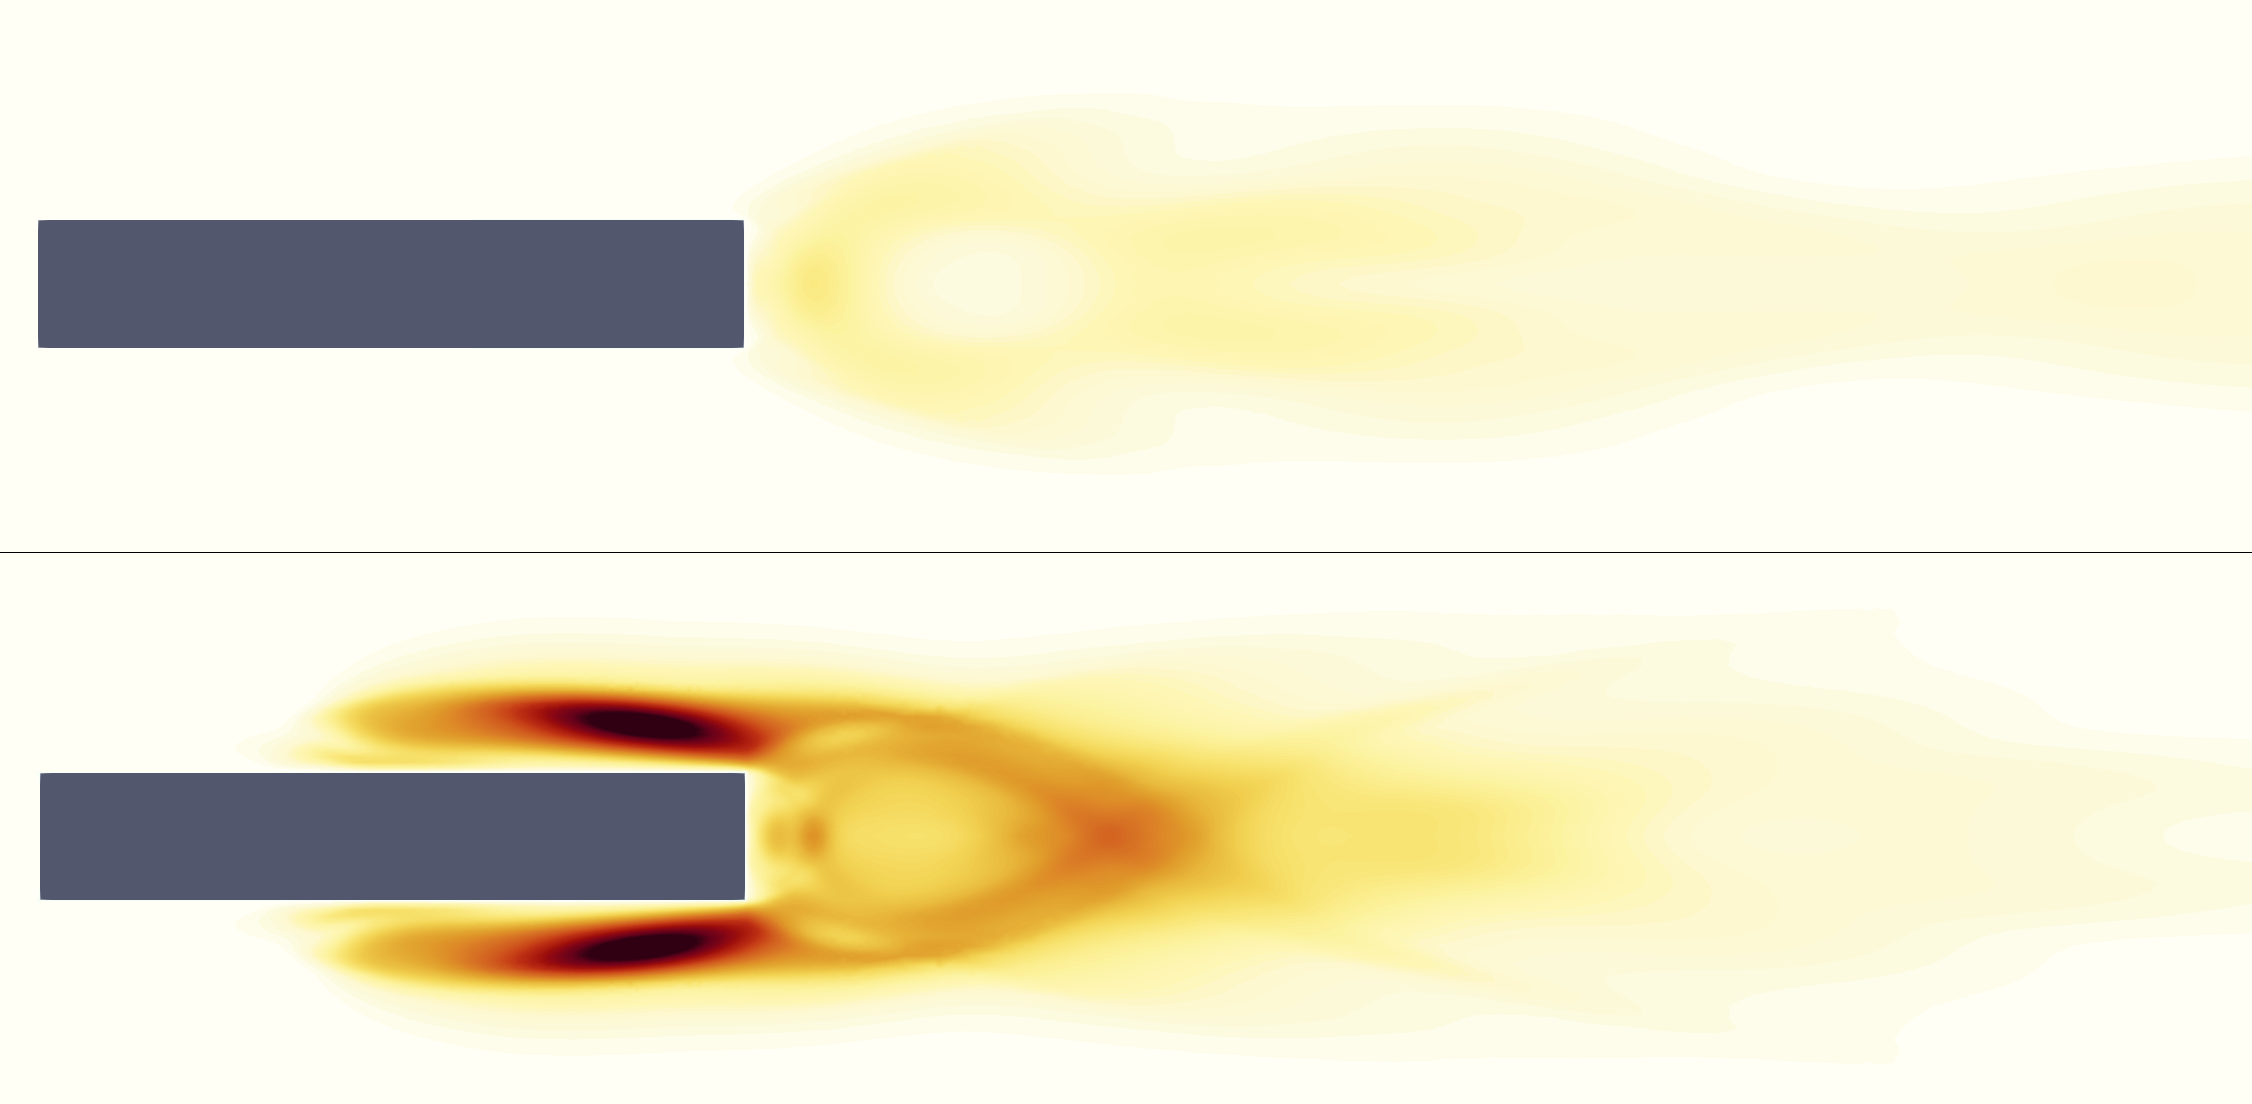
\includegraphics[width=0.49\textwidth]{./fig/AR5s/Ener_AR5p5_Re450_Re550_beta2.png}
  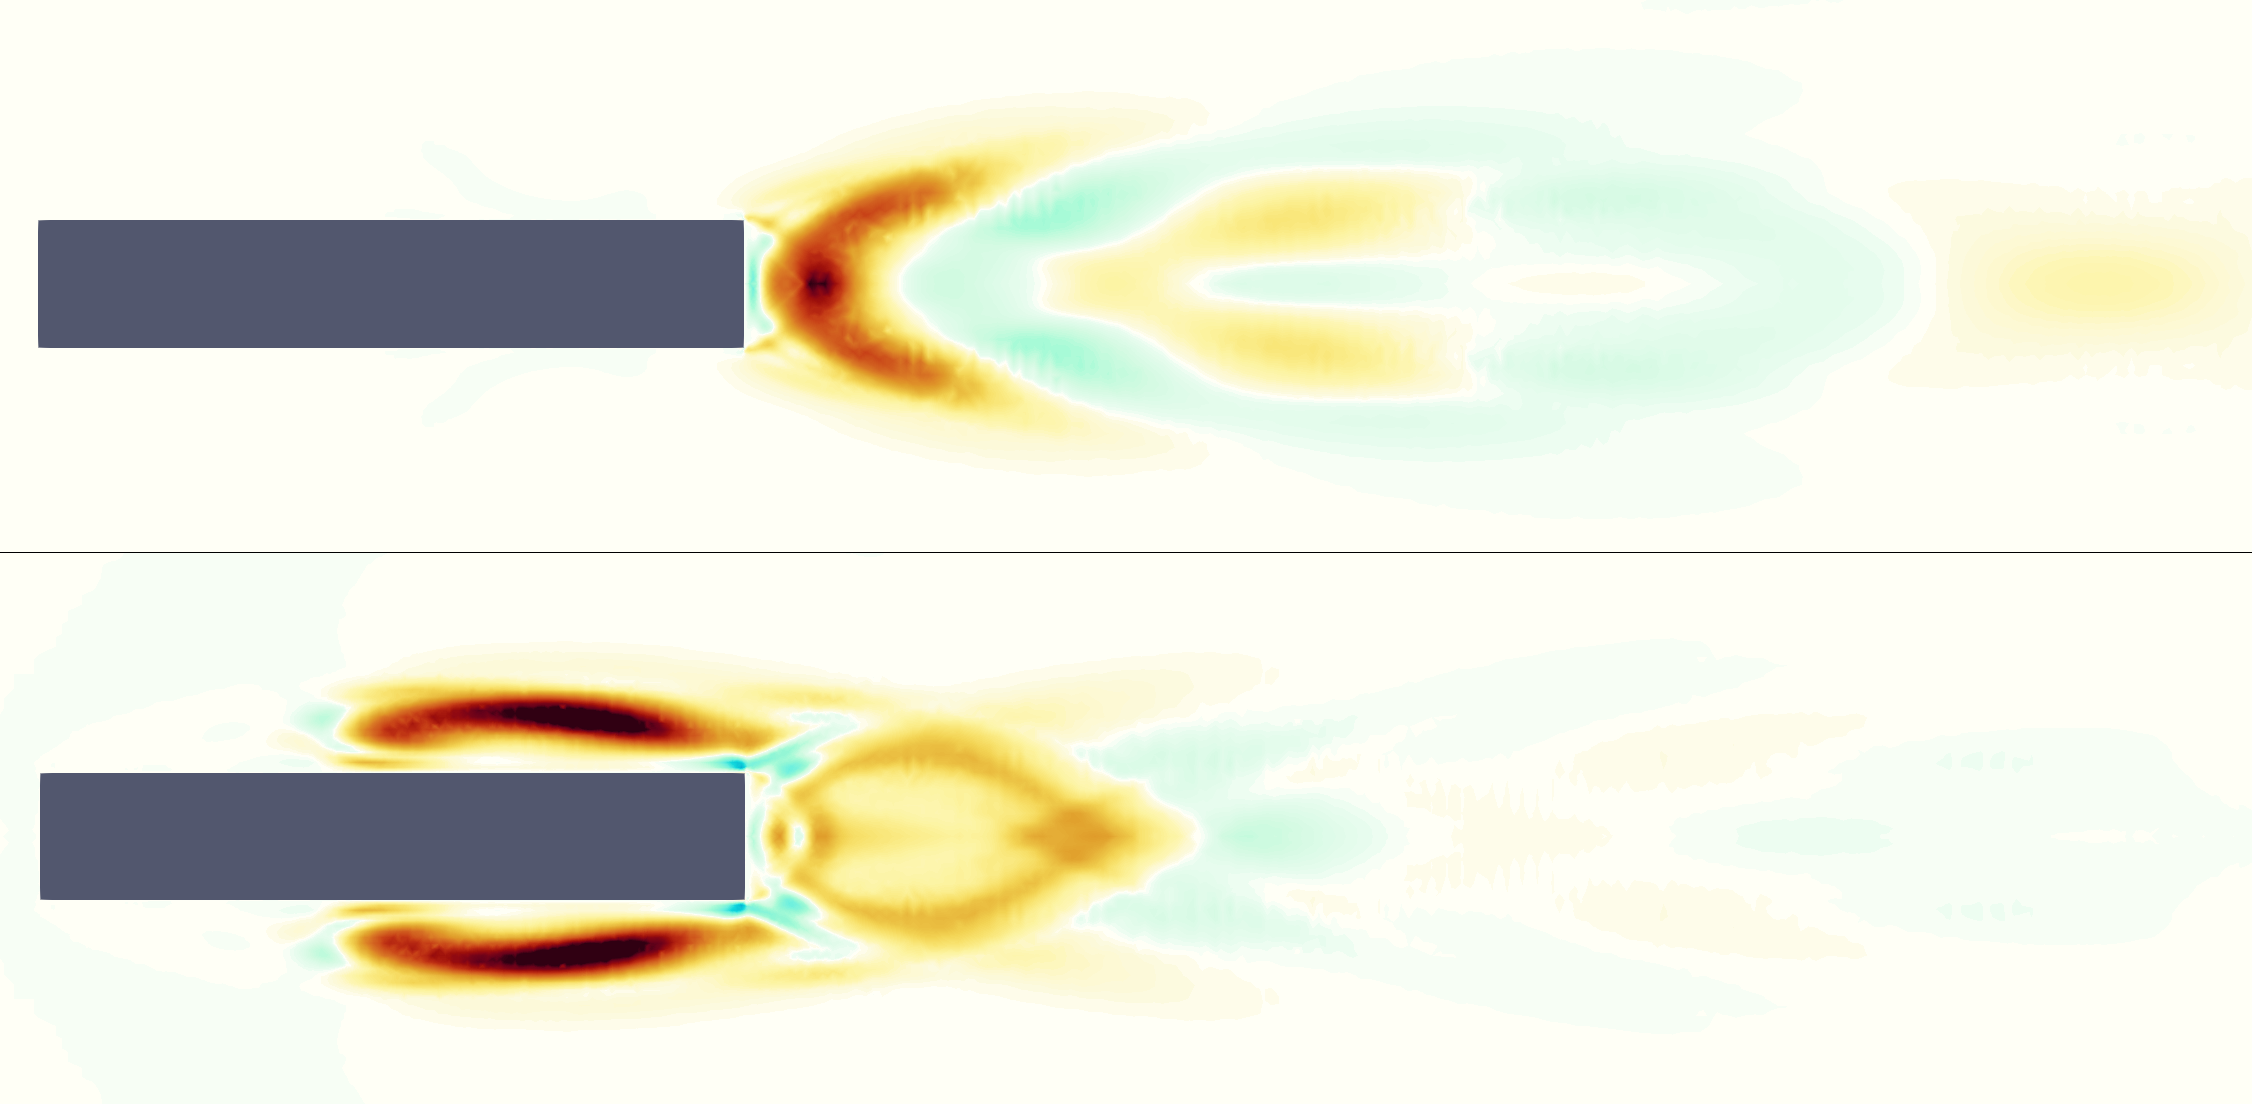
\includegraphics[width=0.49\textwidth]{./fig/AR5s/Prod_AR5p5_Re450_Re550_beta2.png}
  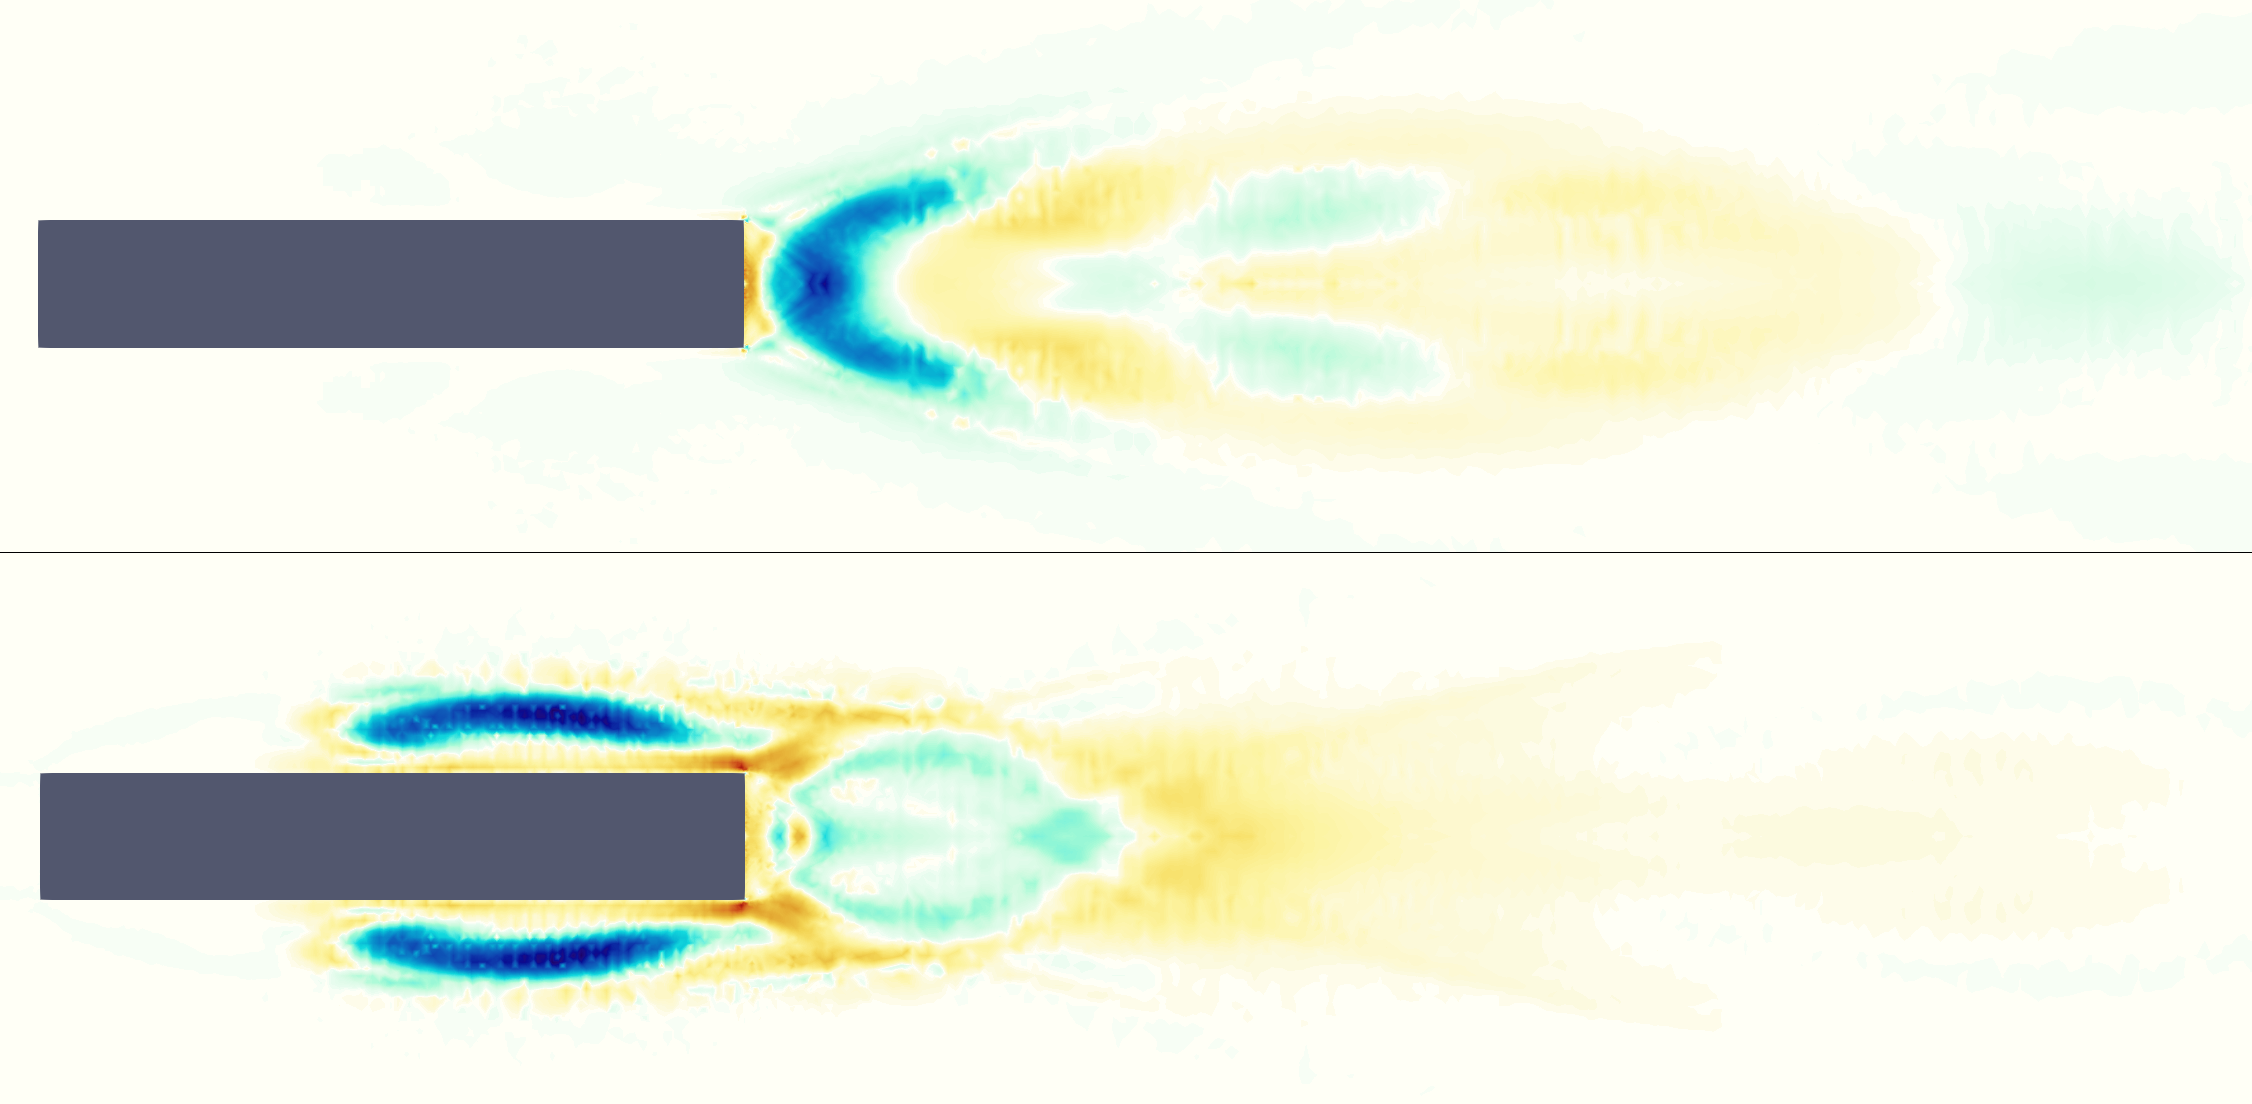
\includegraphics[width=0.49\textwidth]{./fig/AR5s/Trsp_AR5p5_Re450_Re550_beta2.png}
  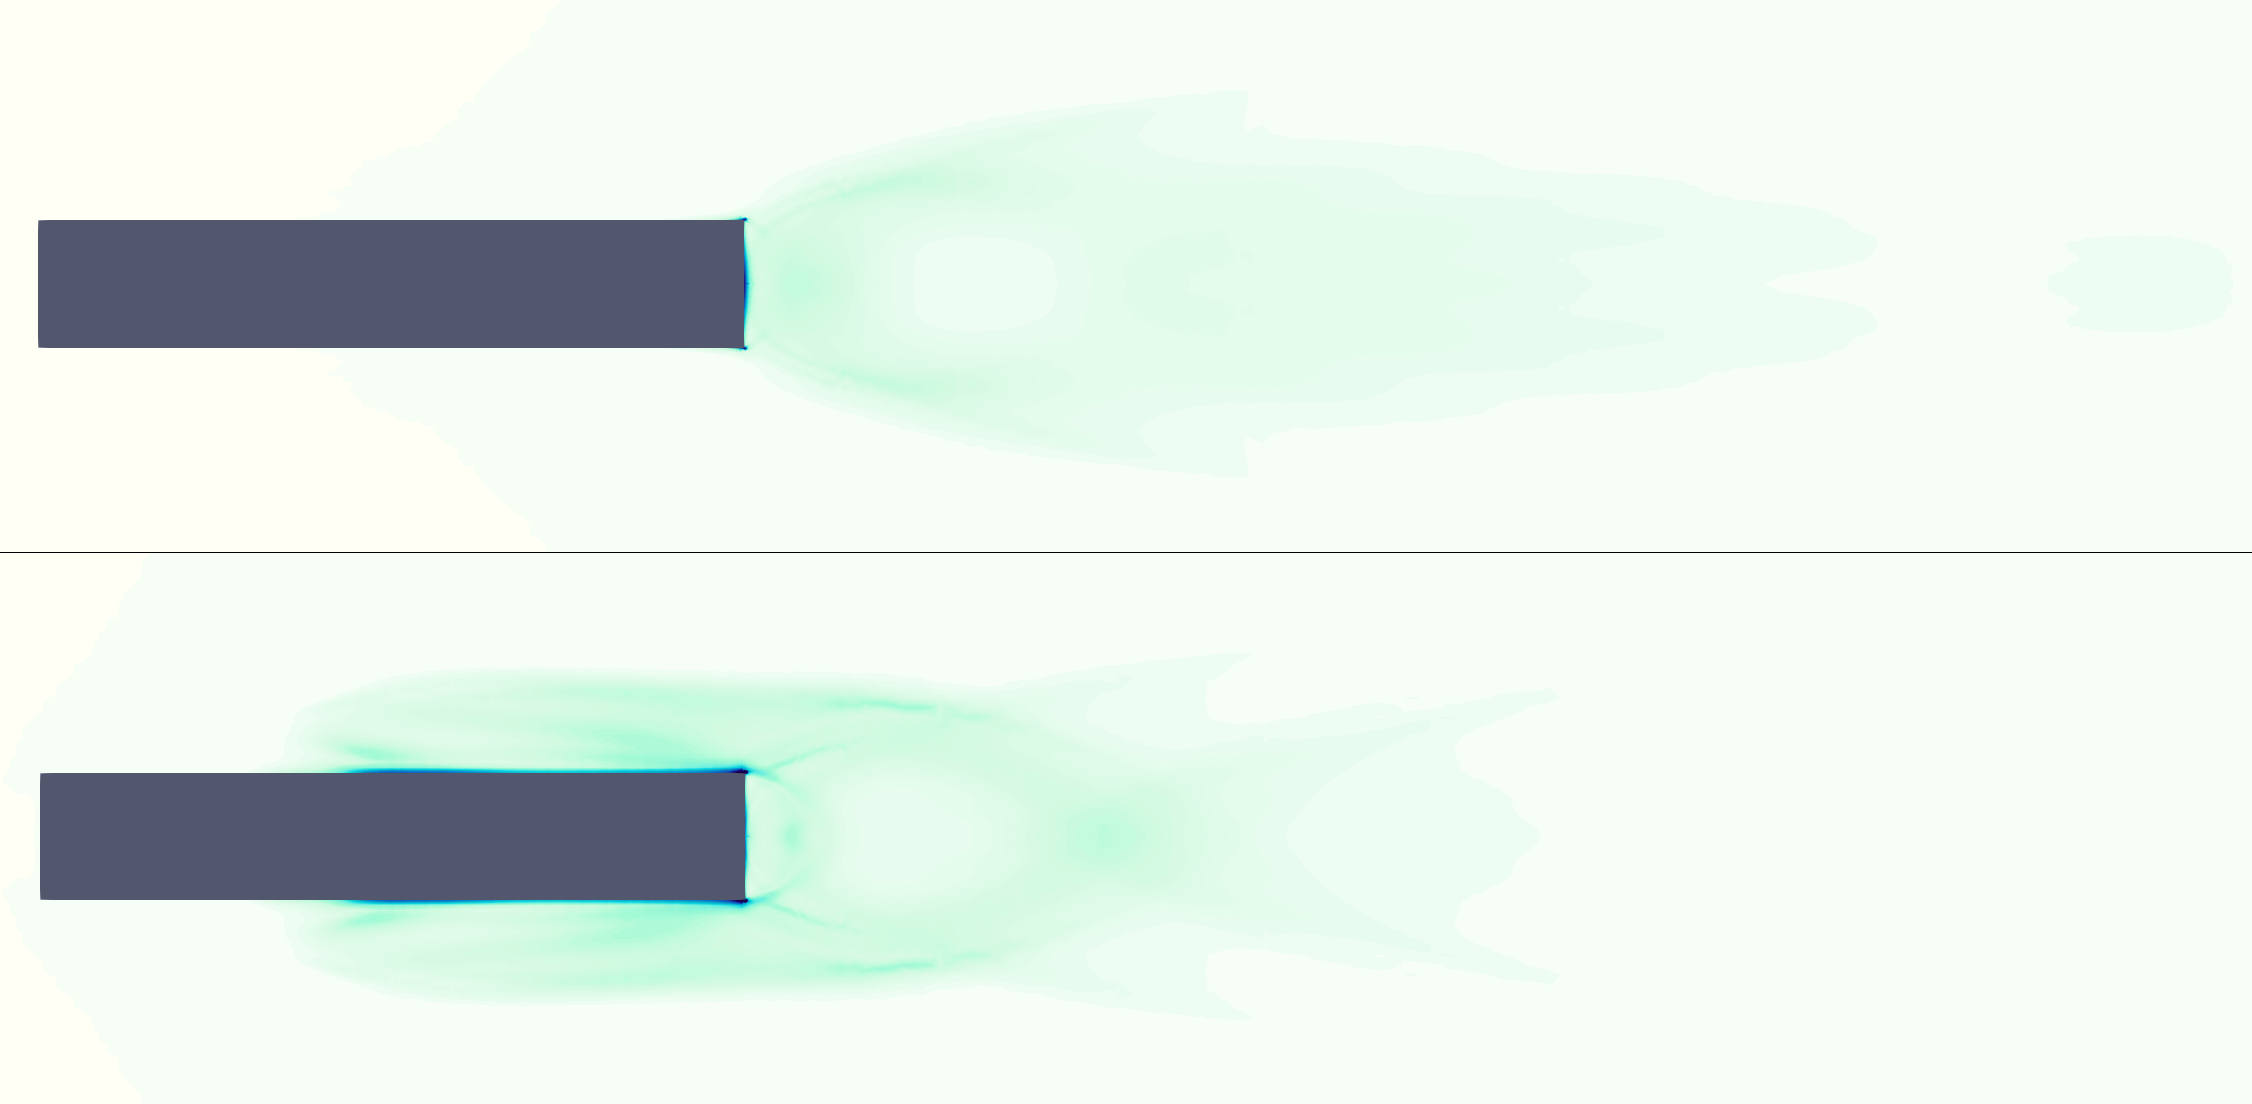
\includegraphics[width=0.49\textwidth]{./fig/AR5s/Diss_AR5p5_Re450_Re550_beta2.png}
  \caption{Budget of energy for mode $A'$ (top) and mode $QS$ (bottom). $\AR=5.5$ and $Re=450$ (for mode $A'$) and $Re=550$ (for mode $QS$). Top left: $u_i u_i^*$. Top right: Production. Bottom left: Transport. Bottom right: Dissipation. XX GUARDARE NELLE DIVERSE ZONE DA COSA VIENE LA CRESCITA. CI SONO DEI TERMINI CHE POSSONO AMPLIFICARE IL MODO (PROD) E ALTRI CHE LO POSSONO LOCALMENTE INVECE DAMPARE, TIPO LA CONVEZIONE. PUò PROBABILMENTE AVERE SENSO ANCHE GUARDARE I CONTRIBUTI DEI TERMINI IN MODO SEPARATO. SIA PER LE COMPONENTI CHE PER QUANTO RIGUARDA INVECE I DIVERSI TEMRINI DI TRASPORTO. GUARDA MARQUET LEFSHATS PER ENDOGENEITY. NON E' LA STESSA COSA, MA SI POSSONO FARE DEI COMMENTI ANALOGHI. POSSIAMO CALCOLARE ENDOGENEITY PER IL CICLO LIMITE? GUARDARE DOVE LA CRESCITà E' LEGATA PIU AD UN FENOMENO DI PRODUZIONE LOCALE O DI ROBA CNVETTIVA XX. PLOTTA SOPRA IL FLUSSO BASE. POSSIAMO ANCHE VEDERE EFFETTO DEL RE. FARE STESSA FIGURA AL VARIARE DEL RE IN MODO QUANTITATIVO. VEDI FIG 8 DI MAEQUT}
  \label{fig:budget_ener}
\end{figure}


\begin{figure}
  \centering
  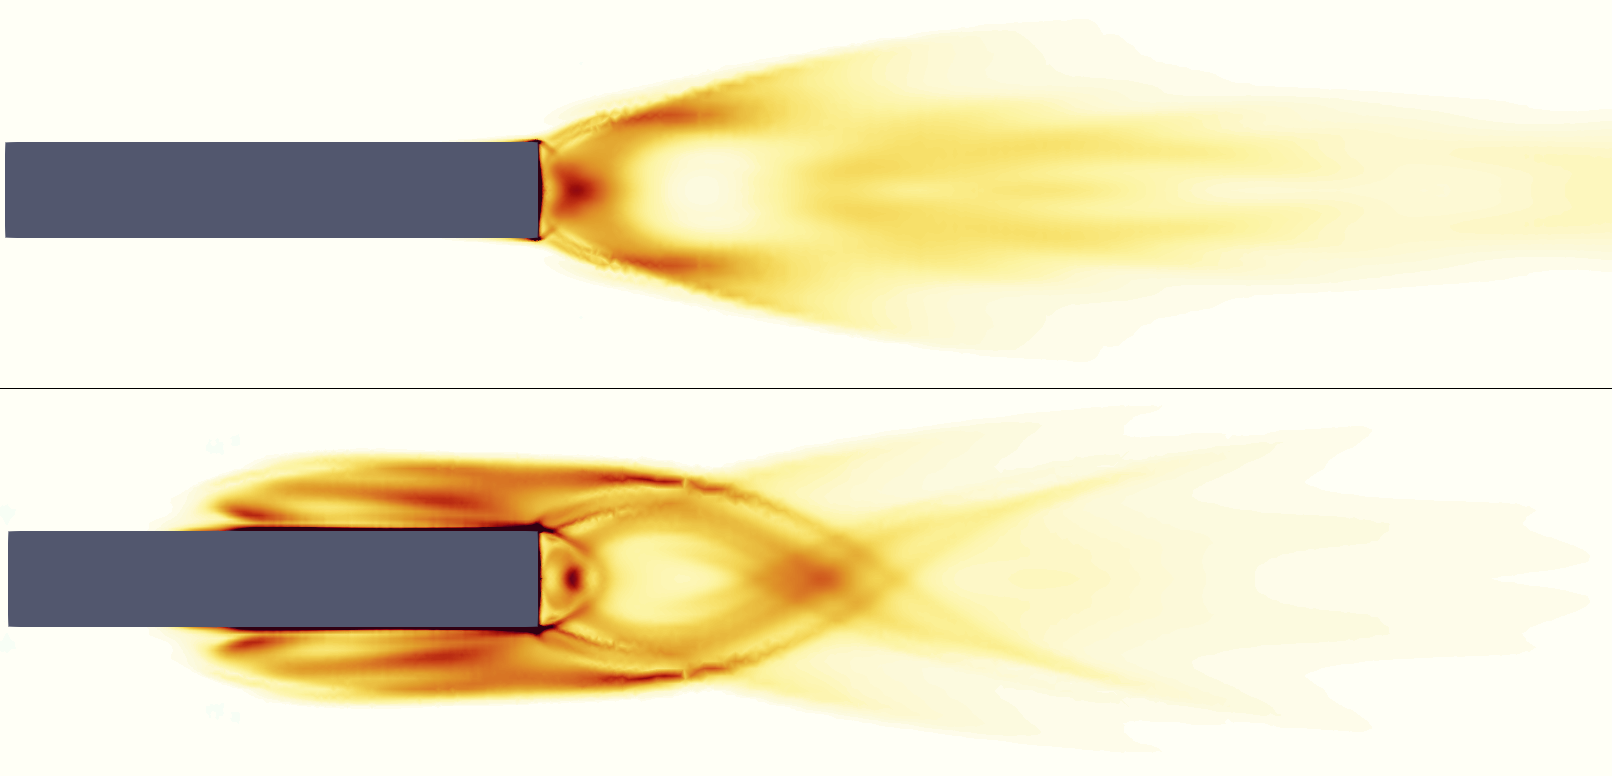
\includegraphics[width=0.49\textwidth]{./fig/AR5s/Enst_AR5p5_Re450_Re550_beta2.png}
  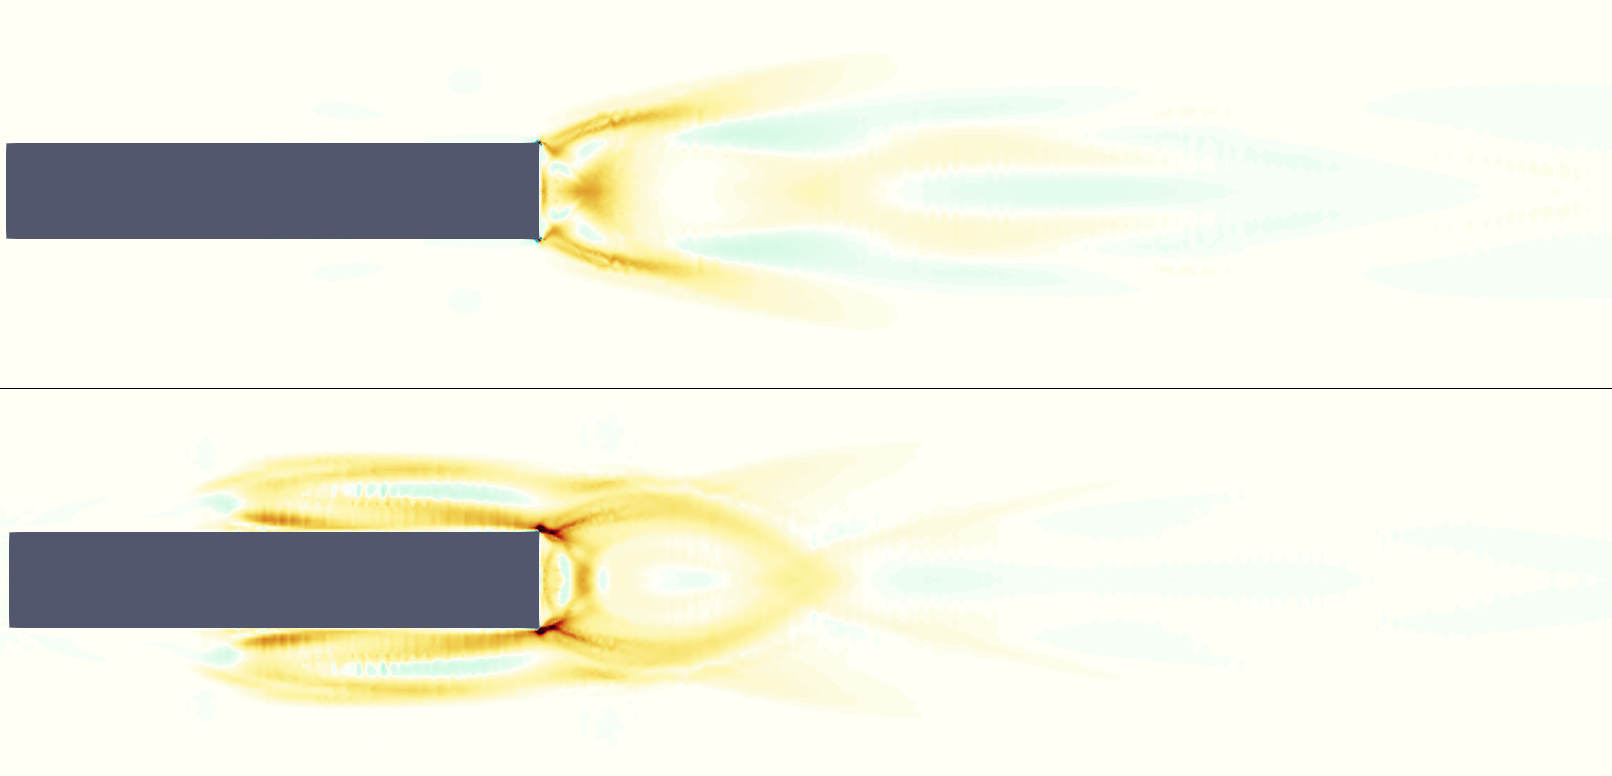
\includegraphics[width=0.49\textwidth]{./fig/AR5s/ProdEnst_AR5p5_Re450_Re550_beta2.png}
  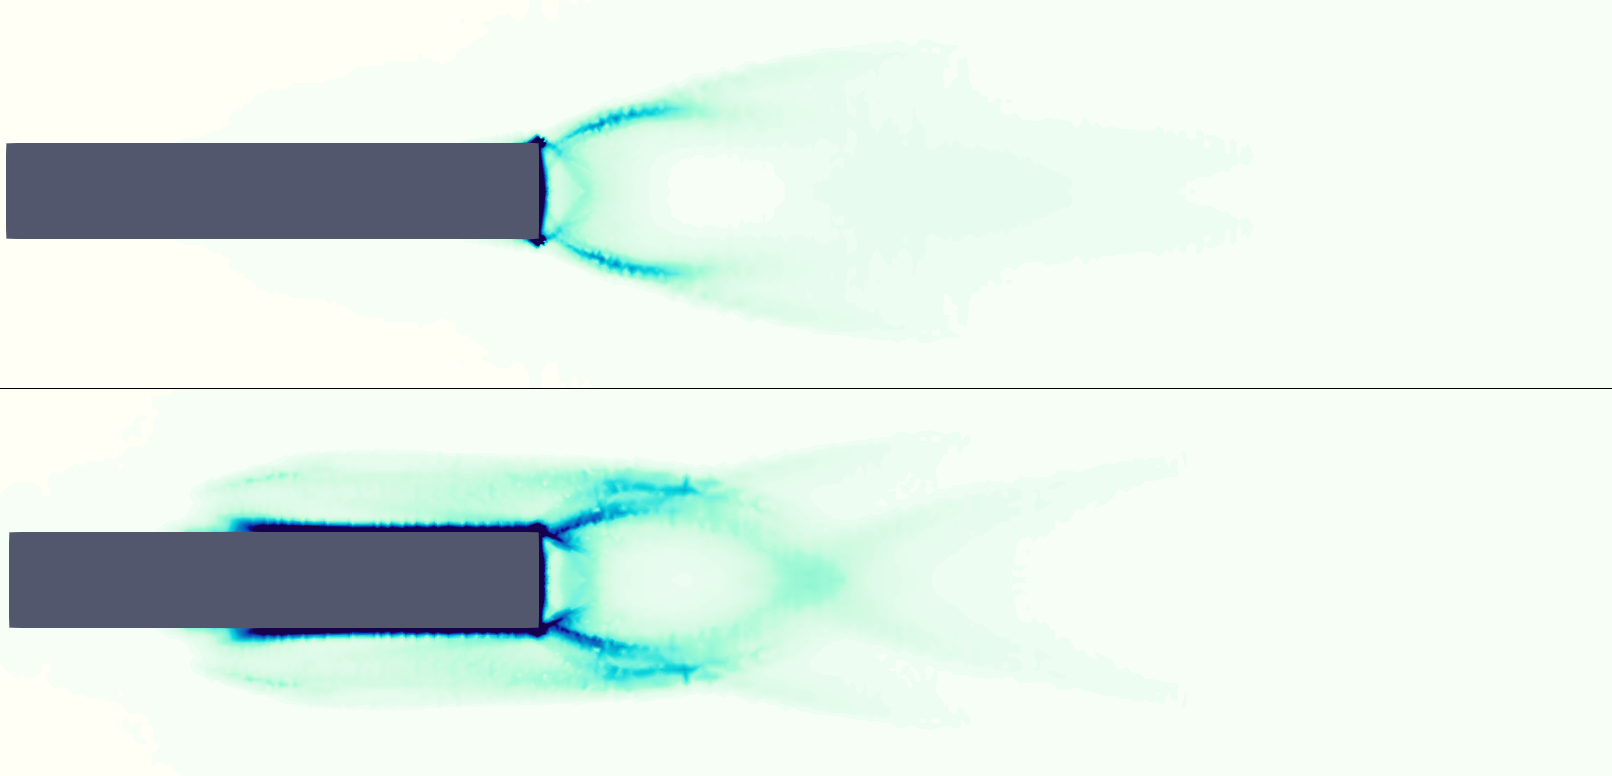
\includegraphics[width=0.49\textwidth]{./fig/AR5s/DissEnst_AR5p5_Re450_Re550_beta2.png}    
  \caption{Budget of enstrophy for mode $A'$ (top) and mode $QS$ (bottom). $\AR=5.5$ and $Re=450$ (for mode $A'$) and $Re=550$ (for mode $QS$). Top left: $\hat{\omega}_i \hat{\omega}_i^*$. Top right: Production. Bottom: Dissipation.}
  \label{fig:budget_enst}
\end{figure}  
